\documentclass[tikz,border=4pt]{standalone}
\usepackage{tikz}
\usepackage{amsmath,amssymb}
\usetikzlibrary{arrows.meta,positioning,shapes.geometric,fit,backgrounds,calc}

\definecolor{navy}{HTML}{1A365D}
\definecolor{darkblue}{HTML}{0F294A}
\definecolor{accentblue}{HTML}{2B6CB0}
\definecolor{softblue}{HTML}{EBF8FF}
\definecolor{darkgreen}{HTML}{22543D}
\definecolor{softgreen}{HTML}{F0FFF4}
\definecolor{darkgray}{HTML}{2D3748}

\begin{document}
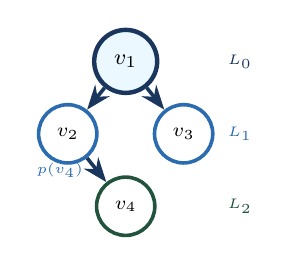
\begin{tikzpicture}[
    scale=0.92,
    >=Stealth,
    font=\sffamily,
    treeNode/.style={circle, draw=navy, fill=white, line width=1.3pt, minimum size=0.74cm, inner sep=0pt, font=\bfseries\scriptsize},
    rootNode/.style={circle, draw=navy, fill=softblue, line width=1.6pt, minimum size=0.80cm, inner sep=0pt, font=\bfseries\footnotesize},
    treeEdge/.style={->, line width=1.3pt, draw=navy}
]

    % Mini tree diagram
    \node[rootNode] (t_v1) at (1.2, 1.9) {$v_1$};
    \node[treeNode, draw=accentblue] (t_v2) at (0.4, 0.9) {$v_2$};
    \node[treeNode, draw=accentblue] (t_v3) at (2.0, 0.9) {$v_3$};
    \node[treeNode, draw=darkgreen] (t_v4) at (1.2, -0.1) {$v_4$};

    \draw[treeEdge] (t_v1) -- (t_v2);
    \draw[treeEdge] (t_v1) -- (t_v3);
    \draw[treeEdge] (t_v2) -- (t_v4) node[midway, left=1pt, font=\tiny\bfseries, text=accentblue] {$p(v_4)$};

    % Level labels on right
    \node[right=2pt, font=\tiny\bfseries, text=navy] at (2.4, 1.9) {$L_0$};
    \node[right=2pt, font=\tiny\bfseries, text=accentblue] at (2.4, 0.9) {$L_1$};
    \node[right=2pt, font=\tiny\bfseries, text=darkgreen] at (2.4, -0.1) {$L_2$};

\end{tikzpicture}
\end{document}
